% Chapter Performance Evaluation

\chapter{Performance Evaluation} % Main chapter title
\label{performance} % For referencing the chapter elsewhere, use \ref{performance}

\section{APNA Management Service Microbenchmark}
\subsection{EphID Generation}
\subsubsection{Goal}
The goal of this experiment was to benchmark different function involved in the process of EphID generation and try to get an idea which is the most the expensive function in term of computation time.
\subsubsection{Experimental Setup}
APNA Management service is running on server located in the Z\"urich with the following specification.
\begin{itemize}
    \item \textbf{Processor:} Intel(R) Xeon(R) CPU E5540  @ 2.53GHz
    \item \textbf{Core:} 6
    \item \textbf{RAM:} 8 GB
\end{itemize}
Client is a Raspberry Pi Model 3B with Quad Core 1.2GHz Broadcom BCM2837 64-bit CPU and 1 GB RAM.
\subsubsection{Results}
We can see that in Figure \ref{fig:perf_ephid} certificate generation is the most expensive process as compared host id generation and encrypting host id. This was an expected behavior because certificate generation involves complex asymmetric cryptographic task of signing the certificate. While on other hand encrypting host id involves symmetric cryptography using AES-CBC encryption mode. And as a general rule of thumb asymmetric cryptography is always more expensive than symmetric cryptography.
\begin{figure}[th!!]
\centering
\noindent
\makebox[\textwidth]{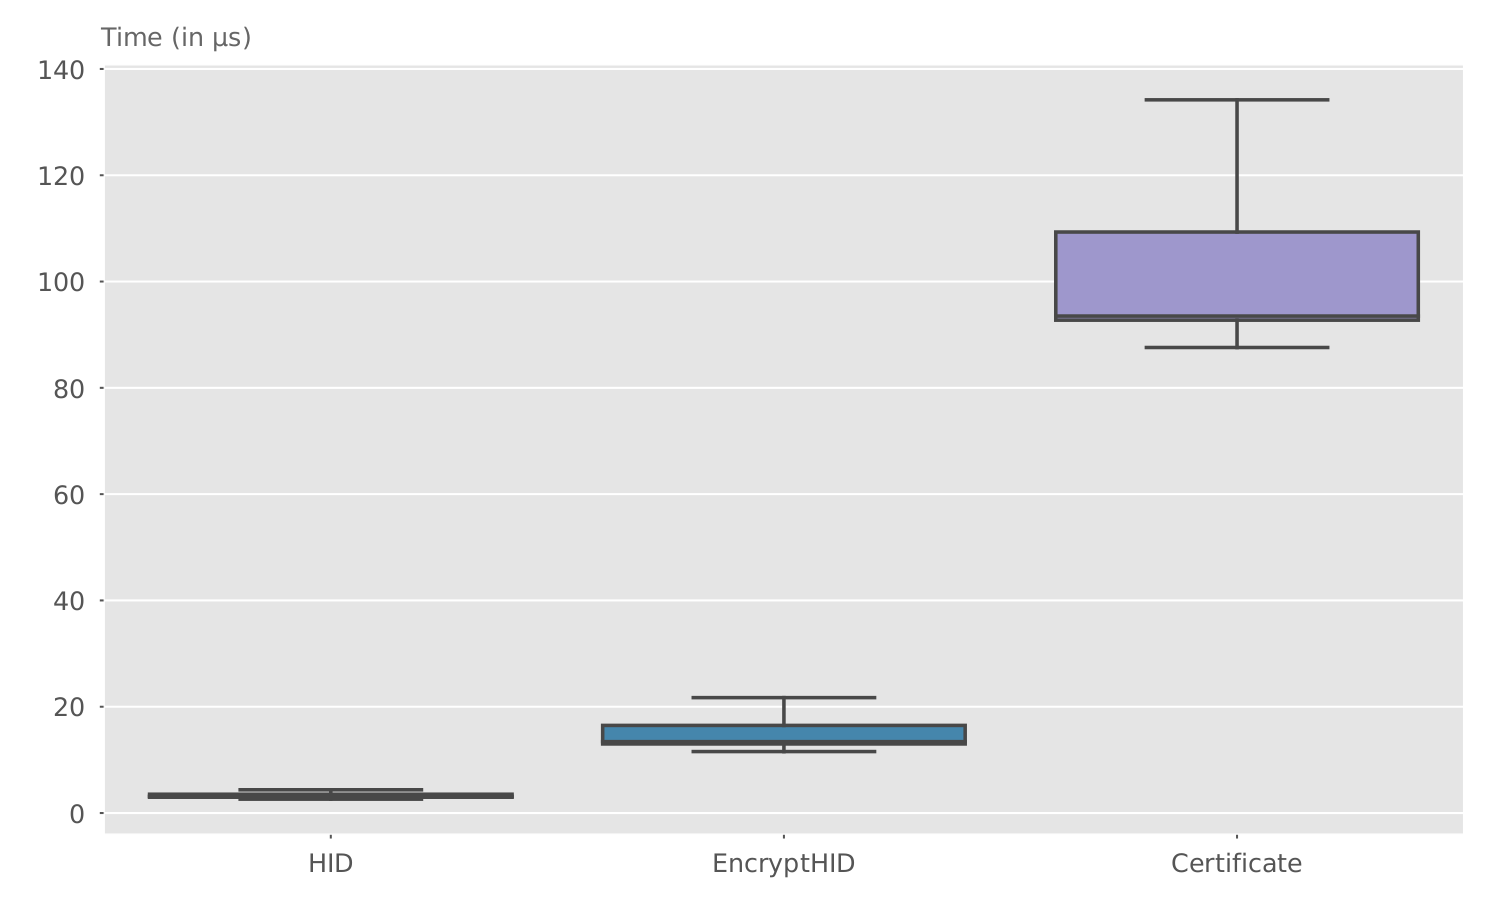
\includegraphics[scale=0.3]{Figures/ephid_gen_stat.png}}
\decoRule
\caption[EphID Generation Ops]{Time taken by different operation involved in EphID generation}
\label{fig:perf_ephid}
\end{figure}

\section{DNS Microbenchmark}

\subsection{Goal}
The Goal of this experiment is to benchmark various operation related to DNS namely: a) DNS Domain Name Registration b) DNS Domain Name Resolution. Currently DNS is implemented using a simple Golang map data structure whose key is the domain name and value is the certificate issued for the Control EphID of the server.

\subsection{Experimental Setup}
There are two different experiments in order to achieve above goal. In the first experiment we are trying to benchmark the rate at which we can register domain names with the DNS Service. 10k domains names were registered with the DNS server while running this experiment. In the second experiment we are trying to benchmark the amount of time DNS server would take to respond to a query if its populated with 10k domain names. Each experiment was repeated 5 times for statistical significance.
\subsubsection{Hardware Specification}
DNS service is running on server located in the Z\"urich with the following specification.
\begin{itemize}
    \item \textbf{Processor:} Intel(R) Core(TM) i7-7820X CPU @ 3.60GHz
    \item \textbf{Core:} 16
    \item \textbf{RAM:} 16 GB
\end{itemize}
Client is a Raspberry Pi Model 3B with Quad Core 1.2GHz Broadcom BCM2837 64-bit CPU and 1 GB RAM.
\begin{figure}[th!!]
\centering
\noindent
\makebox[\textwidth]{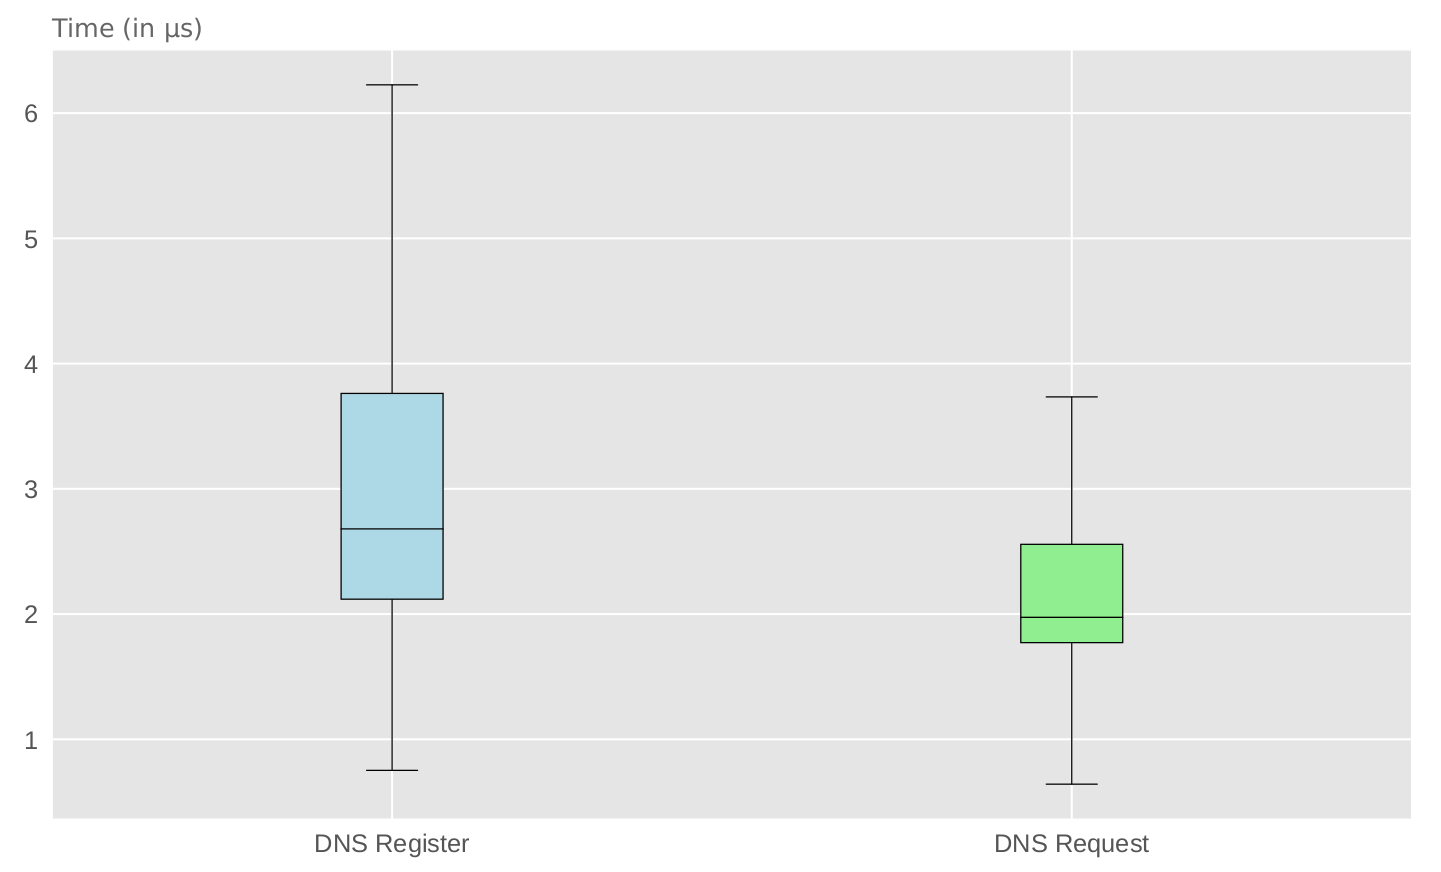
\includegraphics[scale=0.3]{Figures/dns_bench.png}}
\decoRule
\caption[DNS Operations]{Time taken by APNA MS for DNS Register and Request}
\label{fig:perf_dns}
\end{figure}

\subsection{Results}
As we can see in Figure \ref{fig:perf_dns} the amount of time it takes is in the order of few microseconds which is kind of an expected behavior as map inside Golang are implemented as hashmap and thus the complexity of insertion and lookup for hashmap is $\mathcal{O}(1)$ 

\section{Key Management Service Microbenchmark}

\subsection{Goal}
The goal of this experiment is to benchmark key management service of APNA Management Service. Key Management Service performs two major functions namely a) register host symmetric key b) reply to border router/APNA Service with the host symmetric key. Key Management Service is also implemented using simple Golang map data structure whose key is the host id and value is the symmetric key registered by the host for packet authentication.

\subsection{Experimental Setup}
There are two different experiments in order to achieve above goal. In the first experiment we are trying to benchmark the rate at which we can register domain names with the DNS Service. 10k domains names were registered with the DNS server while running this experiment. In the second experiment we are trying to benchmark the amount of time DNS server would take to respond to a query if its populated with 10k domain names. Each experiment was repeated 5 times for statistical significance.
\subsubsection{Hardware Specification}
DNS service is running on server located in the Z\"urich with the following specification.
\begin{itemize}
    \item \textbf{Processor:} Intel(R) Core(TM) i7-7820X CPU @ 3.60GHz
    \item \textbf{Core:} 16
    \item \textbf{RAM:} 16 GB
\end{itemize}
Client is a Raspberry Pi Model 3B with Quad Core 1.2GHz Broadcom BCM2837 64-bit CPU and 1 GB RAM.

\begin{figure}[th!!]
\centering
\noindent
\makebox[\textwidth]{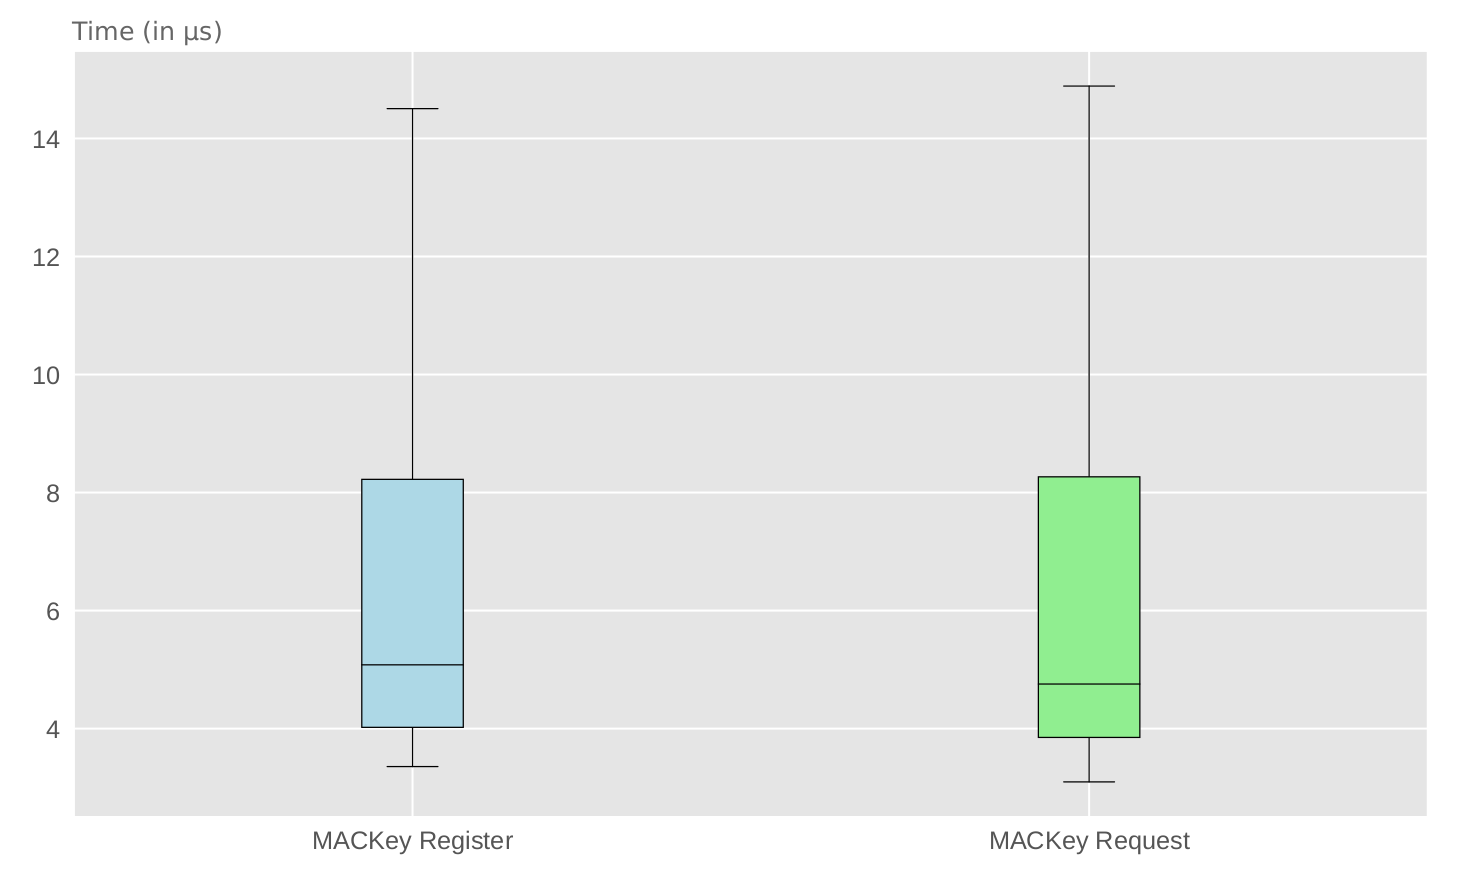
\includegraphics[scale=0.3]{Figures/mac_bench.png}}
\decoRule
\caption[MACKey Operations]{Time taken by APNA MS for MACKey Register and Request}
\label{fig:perf_ephid}
\end{figure}

\section{Host ID}
\begin{figure}[th!!]
\centering
\noindent
\makebox[\textwidth]{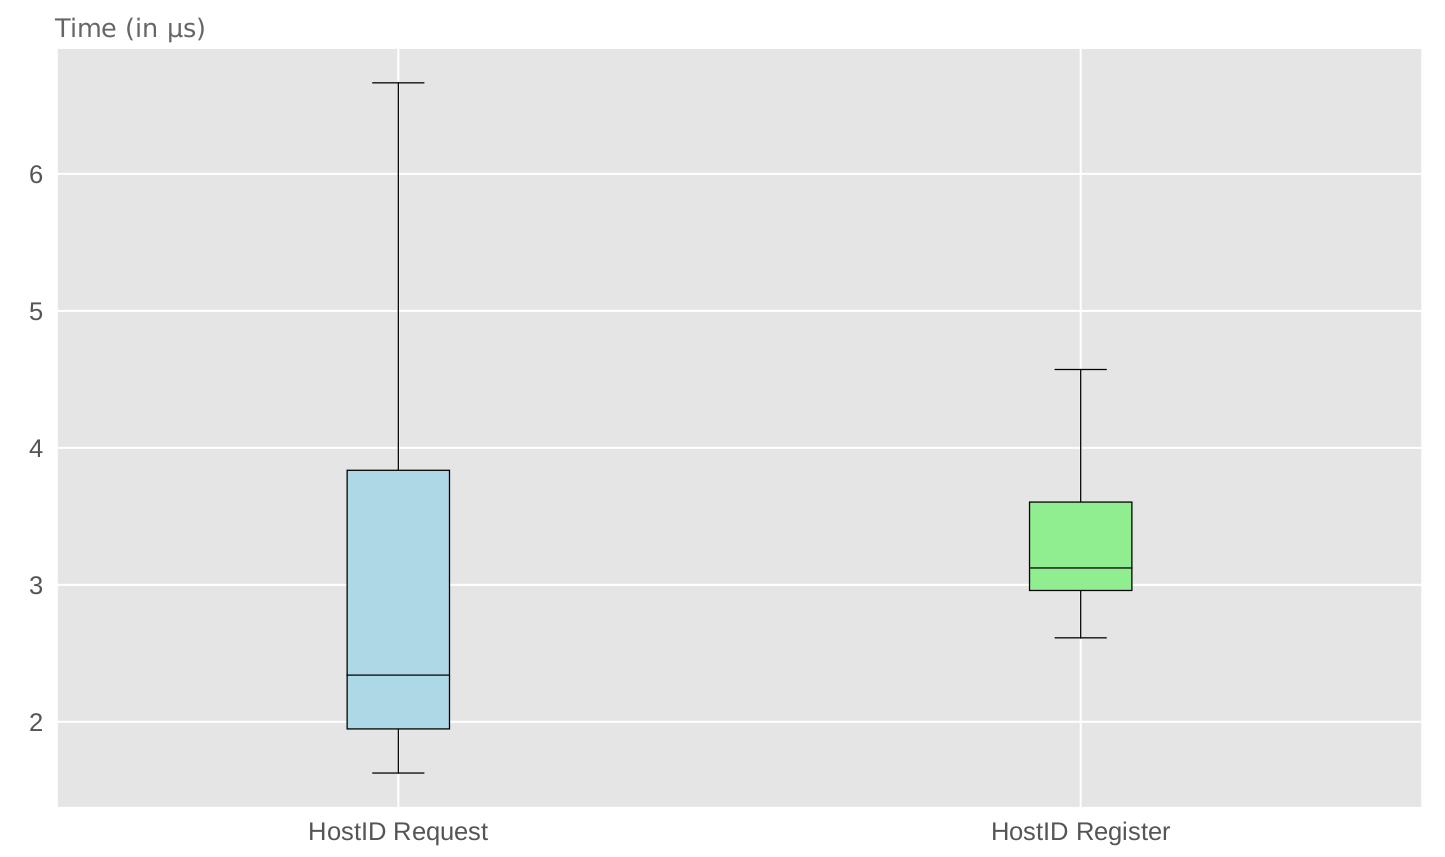
\includegraphics[scale=0.3]{Figures/hid_bench.png}}
\decoRule
\caption[HostID Operations]{Time taken by APNA MS for HostID Register and Request}
\label{fig:perf_ephid}
\end{figure}

\section{Latency}
\begin{figure}[th!!]
\centering
\noindent
\makebox[\textwidth]{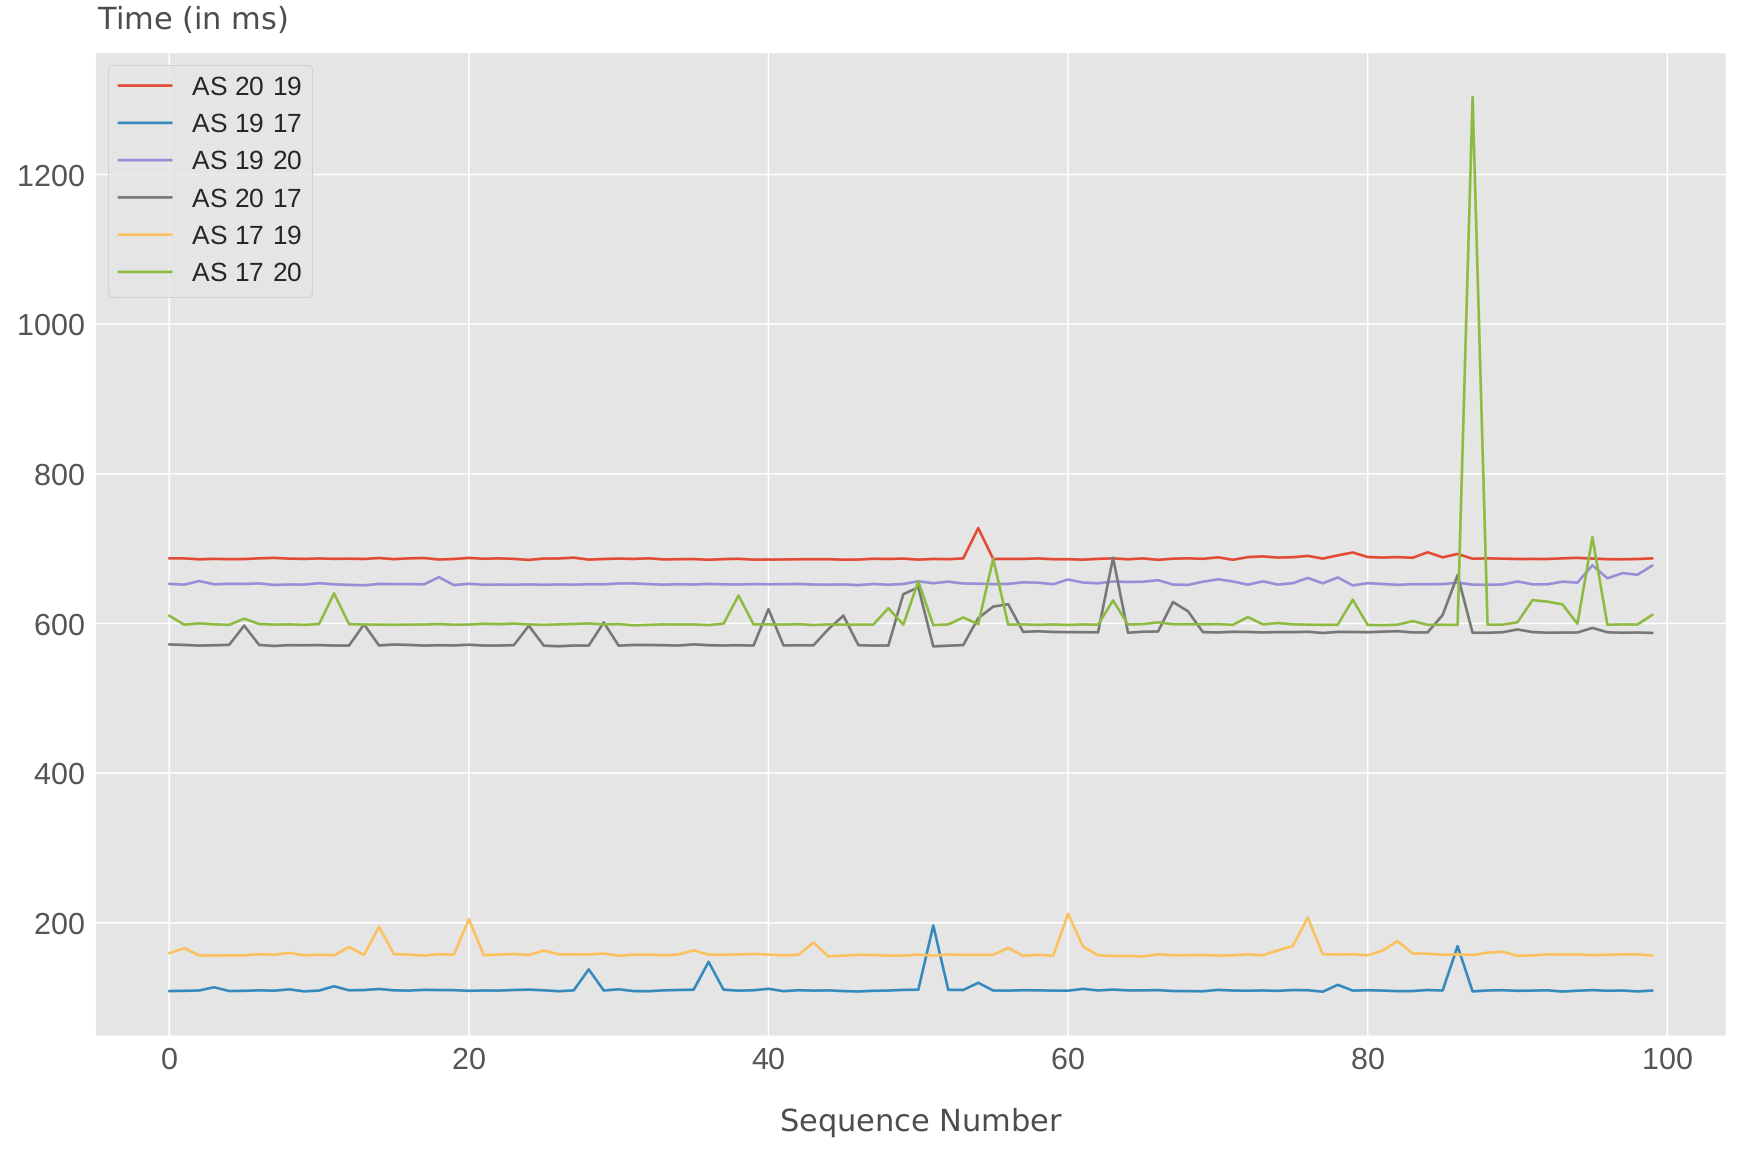
\includegraphics[scale=0.3]{Figures/vanilla_scion_lat.png}}
\decoRule
\caption[Latency Analysis]{Latency Analysis for Vanilla SCION}
\label{fig:perf_ephid}
\end{figure}